\section{CanOp}
\label{sec_CanOp}
CanOp est le nom qui a été donné au projet de crée une sonde nouvelle génération pour la mine Somaïr au Niger. Cette sonde est composée de 3~pièces. 
\begin{itemize}
    \item 2 Sondes de rayonnement Gamma fournissent par la société Geovista
    \item une partie électronique qui inclue une batterie.
    \item Un GPS différentiel fourni par Ophelia 
\end{itemize}
Un opérateur utilise cette sonde en connexion avec une tablette pour déterminer ou extraire du minerai. 
\subsection{Les sondes Gamma}
\label{ssec_sonde}
Les sondes gamma de cet appareil proviennent de chez Ophelia et sont composées de deux parties.
\begin{figure}
    
    \begin{subfigure}{1\textwidth}
        \centering
        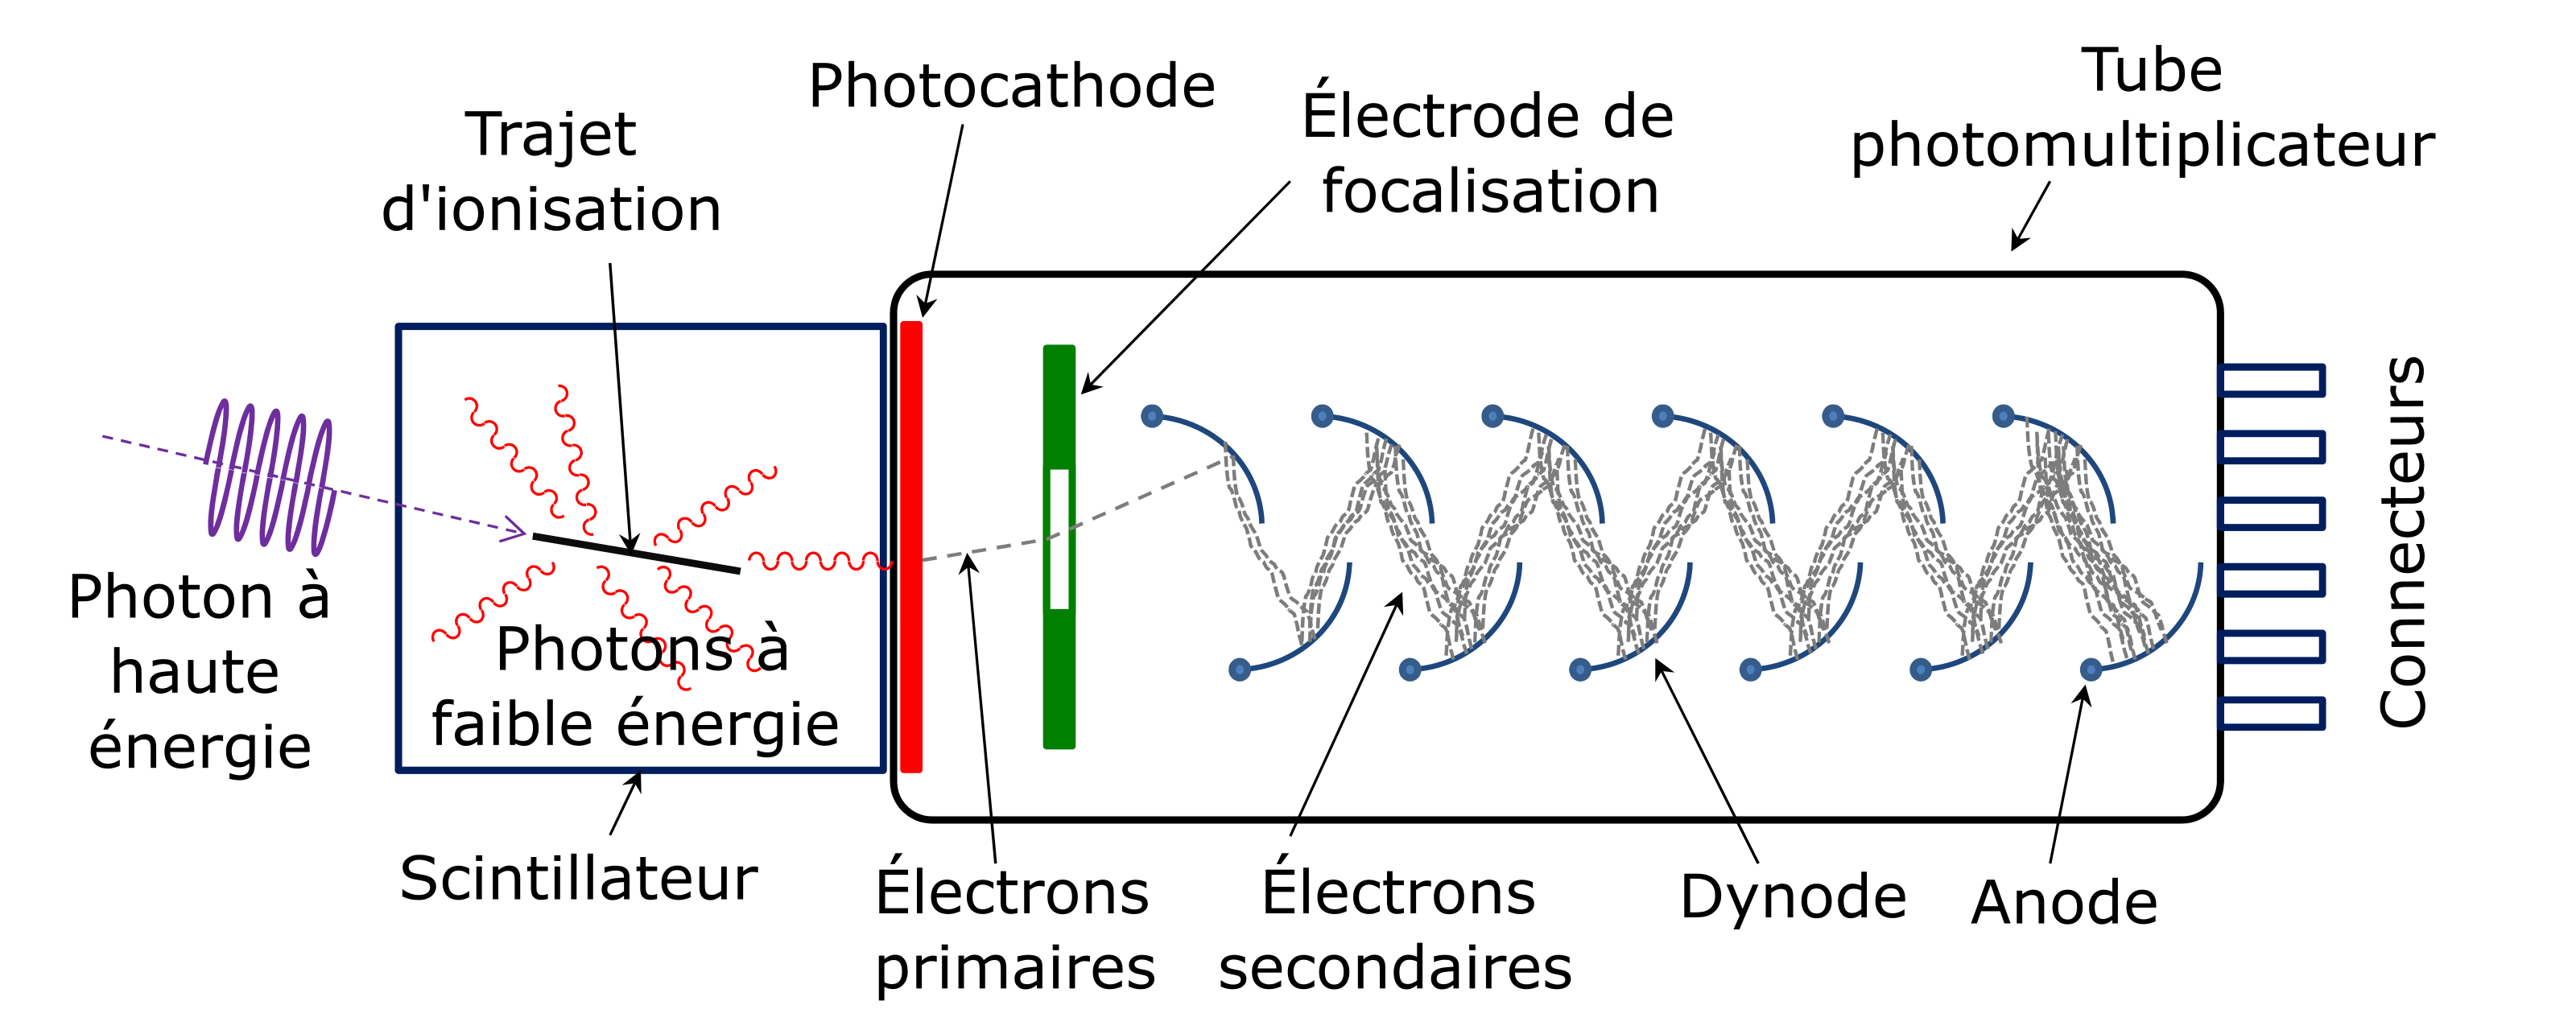
\includegraphics[width=1\textwidth]{img/she/Photomultiplier_coupled_to_a_scintillator_-_fr.png}
        \caption[Shema d'une sonde gamma NaI]{Schéma d'une sonde gamma NaI. Source~: \href{https://commons.wikimedia.org/wiki/File:Photomultiplier_coupled_to_a_scintillator_-_fr.png}{Qwerty123uiop}, \href{https://creativecommons.org/licenses/by-sa/3.0}{CC BY-SA~3.0}, via Wikimedia Commons}
        \label{fig_detecteur_gamma}
    \end{subfigure}
    \begin{subfigure}[t]{0.5\textwidth}
        \centering
        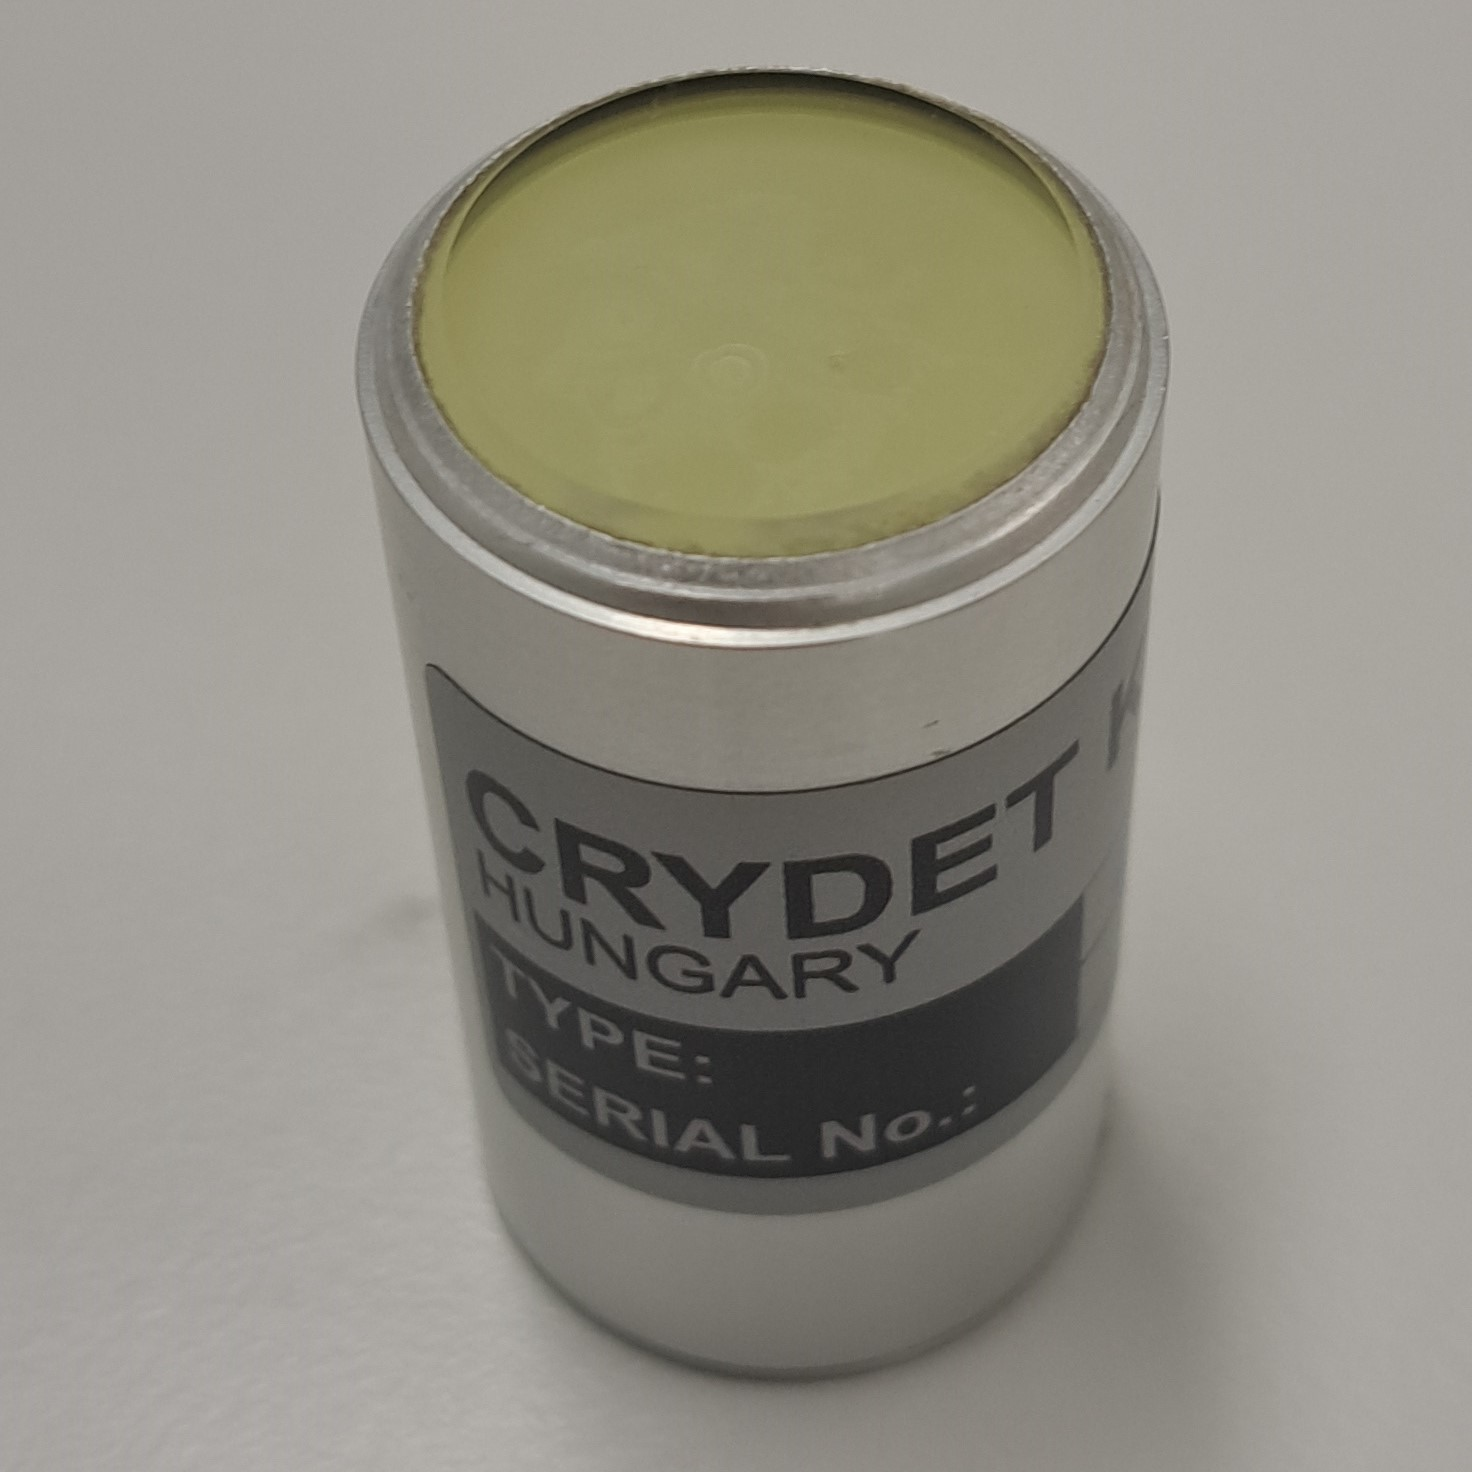
\includegraphics[width=0.9\textwidth]{img/photo/Crystal.jpg}
        \captionsetup{width=.85\textwidth}
        \caption[Photo d'un cristal NaI]{Photo d'un cristal NaI doper au thallium. Dimension~: diamètre 28*50~mm}
        \label{fig_Nai}
    \end{subfigure}
    \begin{subfigure}[t]{0.5\textwidth}
        \centering
        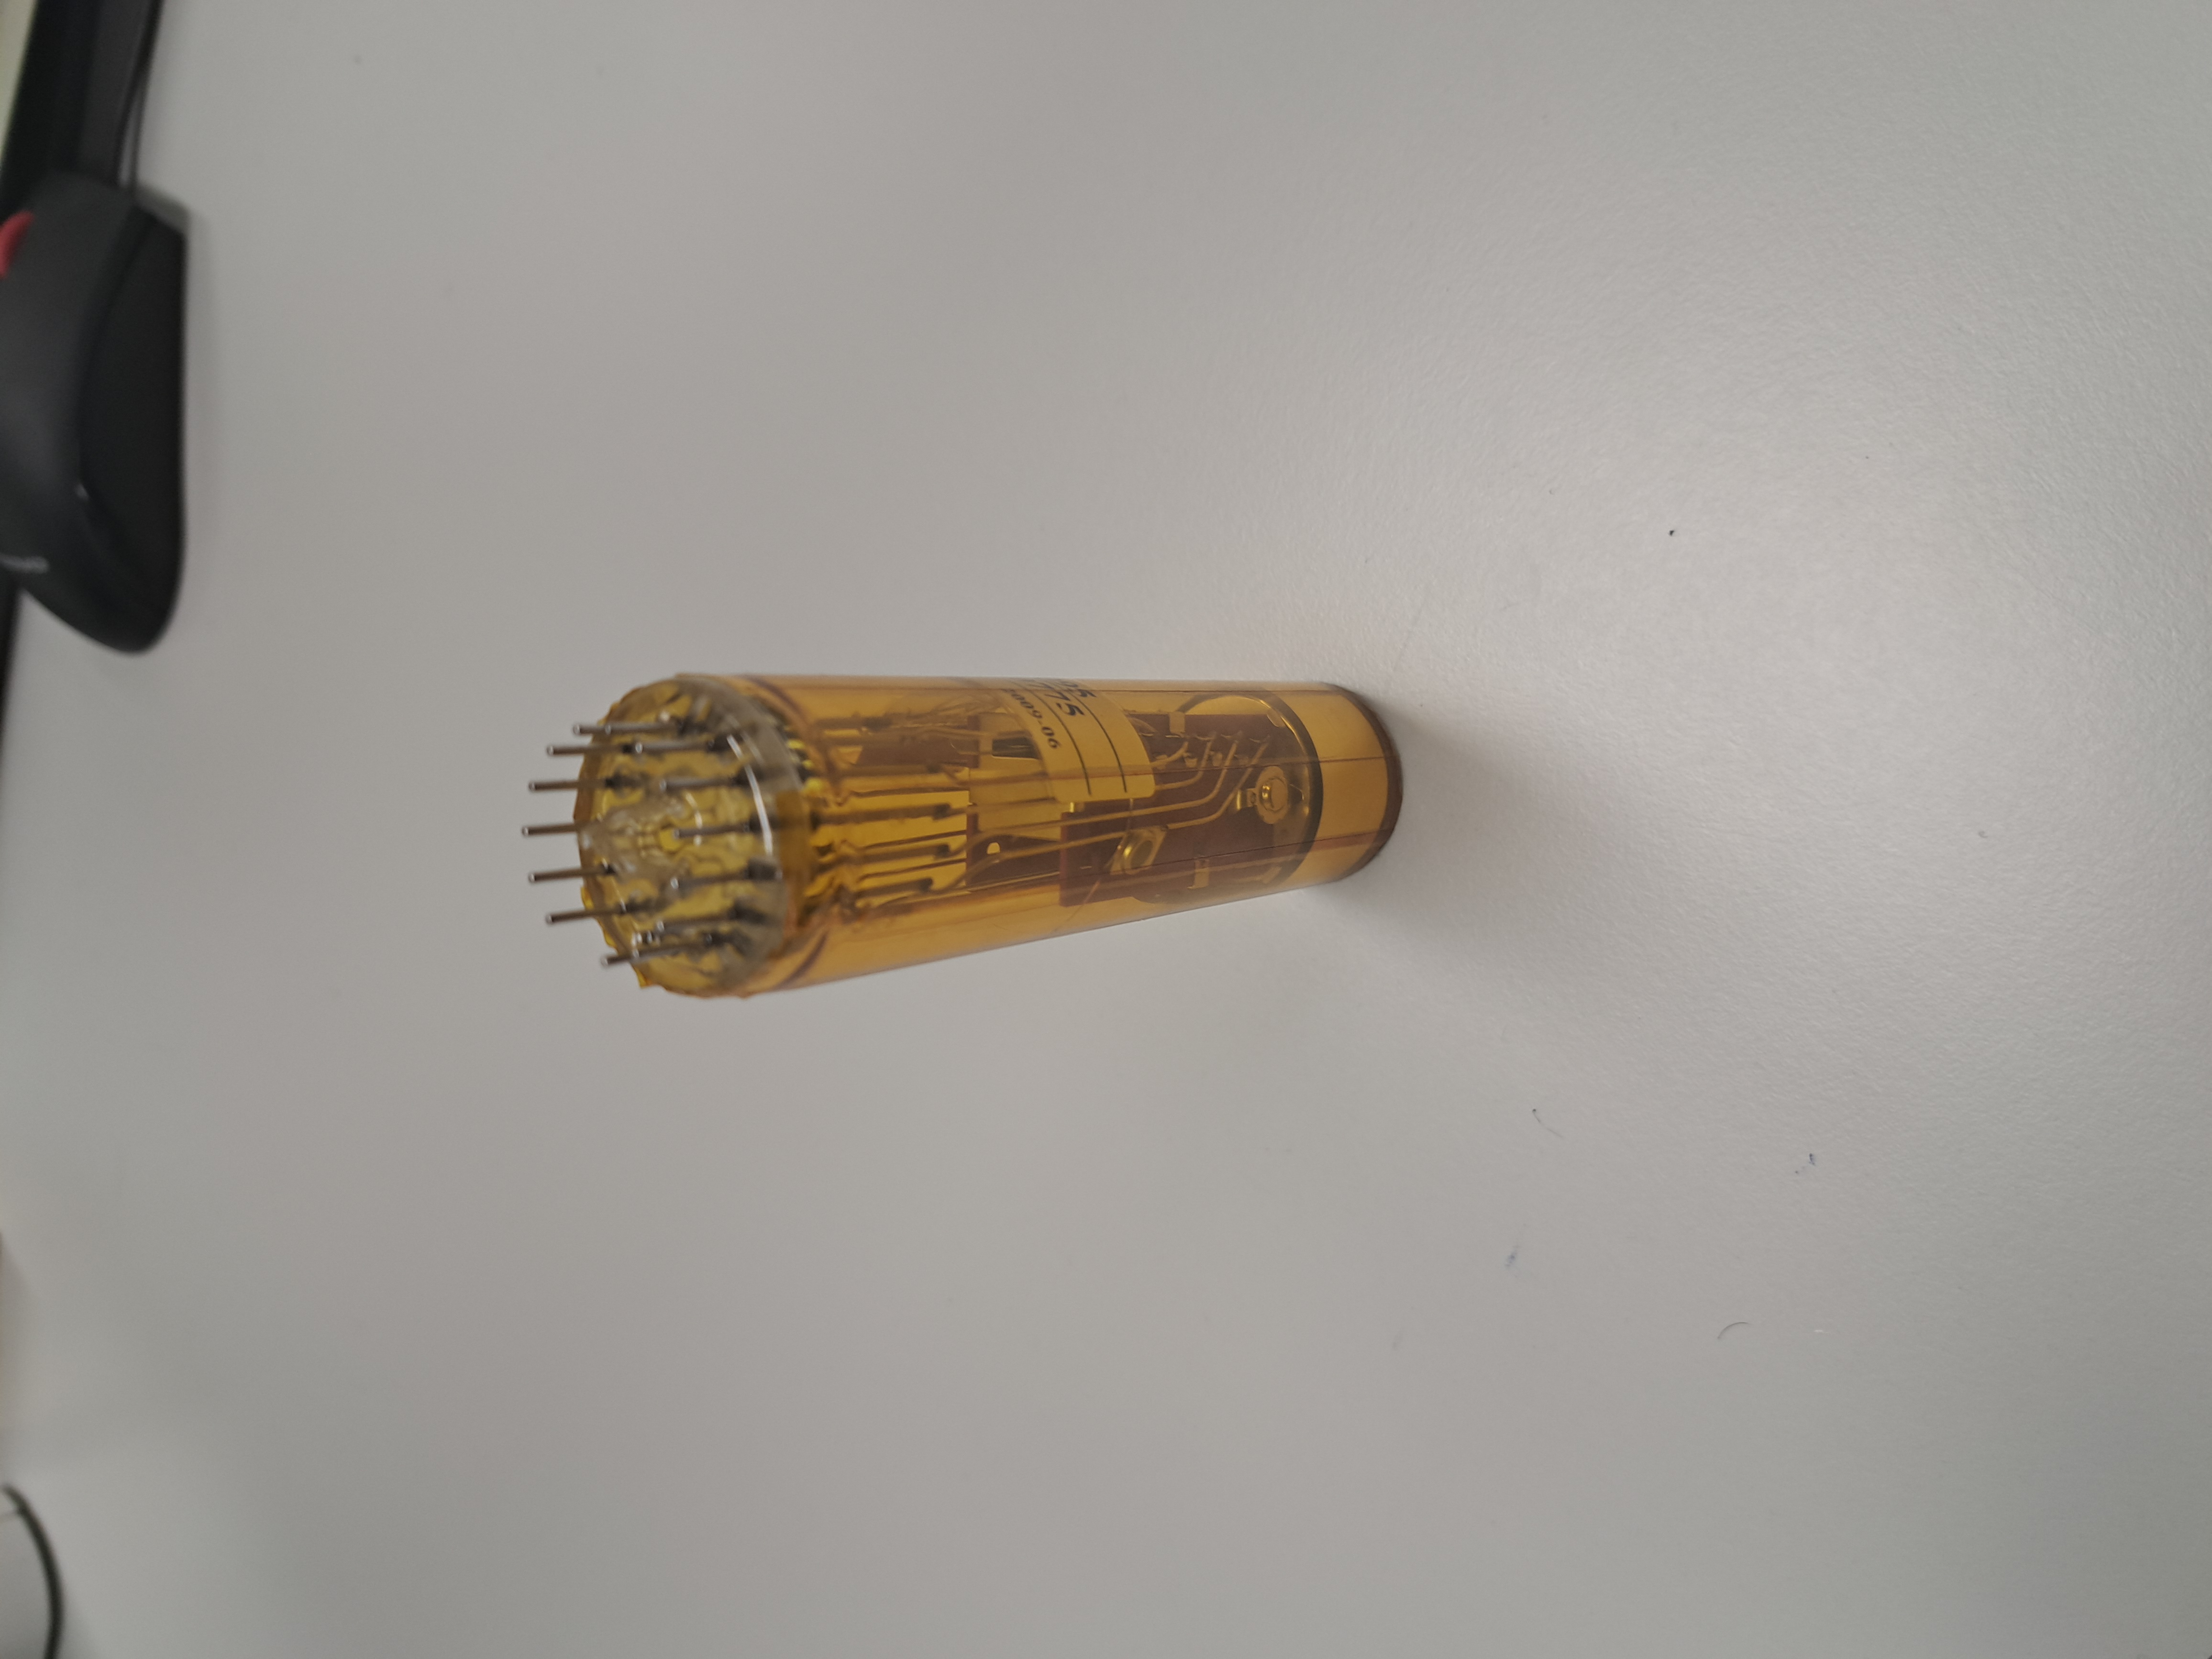
\includegraphics[width=0.9\textwidth]{img/photo/PMT.jpg}
        \captionsetup{width=.85\textwidth}
        \caption[Photo d'un tube photomultiplicateur]{Photo d'un tube photomultiplicateur. Noter la fêlure à gauche de l'étiquette. Dimension~: diamètre 29*114~mm}
        \label{fig_PMT}
    \end{subfigure}
\end{figure}
\begin{description}
    \item[Un crystal NaI] Ce cristal a la propriété d'absorber les photons haut énergie des rayons gamma pour les réémettre comme des photons plus basse énergie (voir partie gauche de la \cref{fig_detecteur_gamma} et \cref{fig_Nai})~\cite{site:explication_NaI}
    \item[Un tube photomultiplicateur]ce tube permet de convertir un photon en un photoélectron qui est ensuite multiplié par le tube pour être converti en signaux électriques. (Voir partie droite de la \cref{fig_detecteur_gamma} et \cref{fig_PMT})~\cite{site:explication_NaI}
\end{description}
À la demande du client (Somaïr), une sonde basse a été incluse dans le projet pour permettre de faire des mesures aux niveaux du sol comme elle était faite avant (voir\ref{}). %photo et section
Les études internes montrent que les mesures les plus fiables sont faites à partir de la sonde haute donc la décision a été prise d'inclure les deux. À l'heure actuel, selon les données enregistrées par la sonde, 68,5~\% des mesures sont faits à partir de la sonde haute et 29~\% à partir de la sonde basse. Les autres mesures sont faites avec une combinaison des deux.

\subsection{Le GPS différentiel}
\label{ssec_Gps_differenciel}
Pour que la CanOp puisse fonctionner correctement, il faut qu'elle soit située très précisément ($\pm$ 10~cm sur les axes x et y et $\pm$ 1~cm sur les axes z), or un GPS classique n'arrive qu’a atteindre $\pm$~3~m horizontalement et $\pm$ 5~m verticalement dus notamment aux perturbations atmosphériques que subisse les signaux. 
\begin{figure}
    \centering
    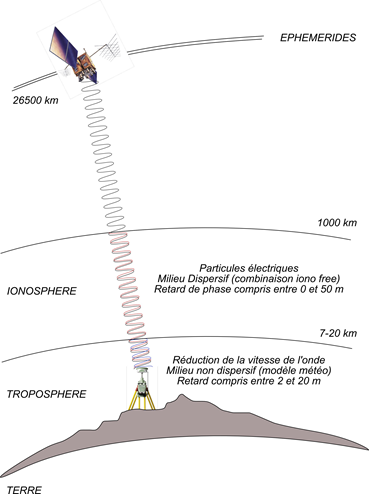
\includegraphics[height=0.5\textwidth]{img/she/GPS-mode-Naturel-5-10m.png}
    \caption[Source d'erreur des GPS]{Schéma présentant les sources d'erreur des GPS. Source~: Orphéon}
    \label{fig_GPS_error_source}
\end{figure}

Une des solutions possibles pour contourner ces problèmes est d'utiliser un GPS différentiel. Le principe de fonctionnement est simple, une station fixe à proximité de notre zone de mesure reçoit également les signaux GPS et en connaissant sa position précise peuvent calculer et transmettre les corrections nécessaires. \cite{site:GPS_diff}
\begin{figure}
    \centering
    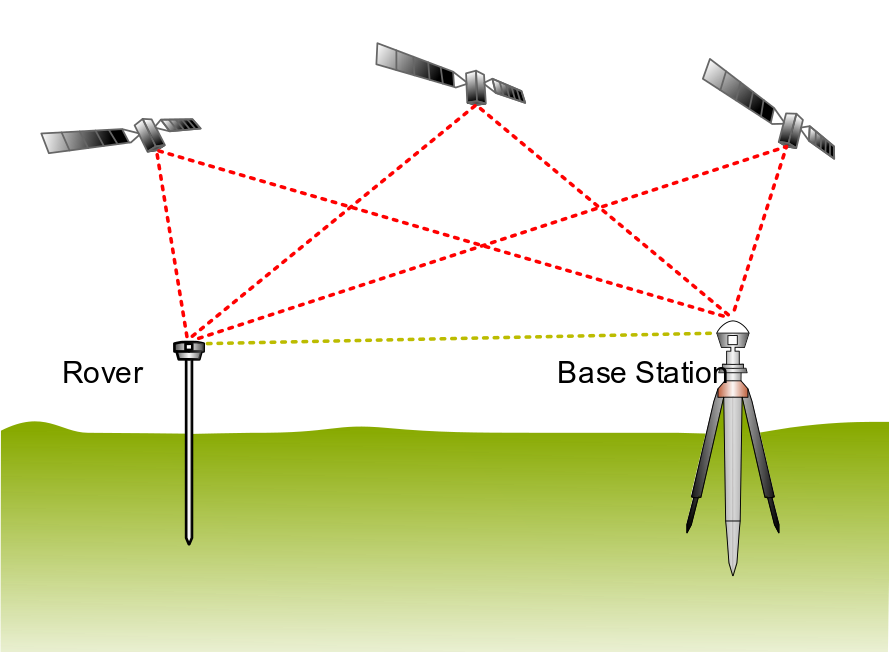
\includegraphics[width=0.5\textwidth]{img/she/Real_time_kinematic.png}
    \caption[Shema d'un systeme GPS differenciel]{Schéma d'un système GPS différentiel. Source~: \href{https://commons.wikimedia.org/wiki/File:Real_time_kinematic.svg}{TS Eriksson}, \href{https://creativecommons.org/licenses/by-sa/4.0}{CC BY-SA~4.0}, via Wikimedia Commons}
    \label{fig_RTK}
\end{figure}

\subsection{L'électronique}

    